\chapter{VC - dimension}

VC stands for the names Varnik--Cherrorenkis. We will be considering a set systems $\mathcal{F}$. And then for a set $X$ we denote $X \cap \mathcal{F}$ as $\{X \cap A : A \in \mathcal{F}\}$.

\section{Set systems}

\begin{defn}
	$\mathcal{F}$ \textbf{breaks} $X$ if $X \cap \mathcal{F} = 2^{X}$.
\end{defn}

Lets see for ourselves an example, which is on picture \ref{broken-x}. For $\mathcal{F}$ we have all half planes in $\R^2$. Then the set $X = \{a,b,c\}$. Then if we draw all lines and choose both planes it will generate $X \cap \mathcal{F} = \{ \emptyset, \{a\}, \{b\}, \{c\}, \{a,b\}, \{b,c\}, \{a,c\}, \{a,b,c\}\}$ which are all subsets of $X$. Hence it breaks the $X$.

\begin{figure}[!ht]\centering
	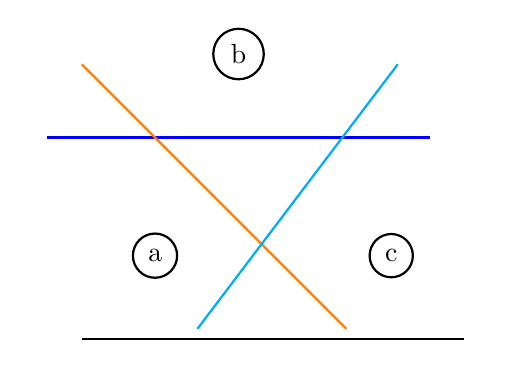
\begin{tikzpicture}[node distance={15mm}, thick, main/.style = {draw, circle}]
		\node (p1) {};
		\node[main] (b) [above right of=p1] {b};
		\node (p2) [below right of=b] {};
		\node[main] (a) [below of=p1] {a};
		\node (p3) [right of=a] {};
		\node[main] (c) [right of=p3] {c};
		\node (1) [left of=p1] {};
		\node (2) [right of=p2] {};
		\node (3) [above right of=p2] {};
		\node (4) [below left of=p3] {};
		\node (5) [above left of=p1] {};
		\node (6) [below right of=p3] {};
		\node (7) [left of=4] {};
		\node (8) [right of=6] {};
		\draw[color=black] (7) -- (8);
		\draw[color=blue] (1) -- (2);
		\draw[color=orange] (5) -- (6);
		\draw[color=cyan] (3) -- (4);
	\end{tikzpicture}
	\caption{Example of $\mathcal{F}$ and set $X$ which is broken.}
	\label{broken-x}
\end{figure}

\begin{defn}
	We say that $VC-\dim(\mathcal{F})$ is $\max \{|X| : \mathcal{F} \text{ breaks } X\}$.
\end{defn}

In our previous example we see that $VC-\dim(\mathcal{F})$ is at least 3. But we may see that it is exactly 3. Because if we take 4 points they are either all in convex hull thus it is impossible to take the opposite points or one point is in the convex hull of other three of them, for which it is impossible to take only the points forming the convex hull except the middle one. Other example can be $\mathcal{F}$ as all intervals in $\R$ for which the $VC-\dim(\mathcal{F})$ is 2.

All these examples are geometrical ones. Lets see some for graph theory. Lets have $G$ graph s.t. $K_{n} \nleq_{t} G$. Then $\mathcal{F} = \{N_{G}[v] : v \in V(G)\}$. Where the \textbf{closed neighborhood} is defined as $N_{G}[v] = \{v\} \cup \{u \mid \{u,v\} \in E(G)\}$. We may see that $VC-\dim(\mathcal{F}) \leq n-1$. For contradiction $X \subseteq V$ and $|X| = n$. For every 2-element subset there is a vertex adjacent to them, this would give me a $K_{n}$ as a topological subgraph.

\section{Subsystems}

Now we will be considering sub-systems. That is $\mathcal{F} \subseteq 2^{Y}$ for some $Y$. There will be defined a measurement $\mu$ on $Y$. As an example can be the half-planes but only inside the square of size 1.

\begin{defn}
	$N$ is an $\epsilon$-net if
	
	$$
	(\forall A \in \mathcal{F}) : \mu(A) \geq \epsilon \mu(Y) \land N \cap A \neq \emptyset
	$$
\end{defn}

For an example consider $\mathcal{F} = \{\text{axis aligned rectangles in }Y\}$ and $\mu$ be the area of the rectangle. Then the $\epsilon$-net must hit all rectangles. We can easily create a grid of points which are $\epsilon$ apart. This will create $\frac{1}{\epsilon^2}$ points in net.

\begin{thm}
	There $\exists c$ s.t. if $\mathcal{F} \subseteq 2^Y$ has $VC-\dim(\mathcal{F})$ $k$ then
	
	$$
	(\forall \epsilon > 0) c \frac{k}{\epsilon} \log \left( \frac{k}{\epsilon} \right)
	$$
	
	independently at random chosen elements of $Y$ form an $\epsilon$-net with probability $\geq 1/2$. This is all with the probability for $A \subseteq Y$ $\Pr [p \in A] = \frac{\mu(A)}{\mu(Y)}$.
\end{thm}

\begin{defn}
	$\tau (\mathcal{F}) = \min \left( |Z| : (\forall A \in \mathcal{F}) Z \cap A \neq \emptyset \right)$.
\end{defn}

As an example we may see that for $\mathcal{F}$ closed neighborhood in $G$ the $\tau(\mathcal{F})$ is for the minimal size of dominating set in the given graph $G$.